%!TEX root = main.tex

\section{Real-World Regular Expressions}\label{sec-rwre}


Throughout the paper, $\Int^+$ denotes the set of positive integers, and  $\nat$ denotes the set of natural numbers. Furthermore, for $n\in \Int^+$, let $[n]:=\{1, \ldots, n\}$. 

We use $\Sigma$ to denote a finite set of letters, called \emph{alphabet}. A \emph{string} over $\Sigma$ is a finite sequence of letters from $\Sigma$. We use $\Sigma^*$ to denote the set of strings over $\Sigma$ and $\varepsilon$ to denote the empty string. Moreover, for convenience, we use $\Sigma^\varepsilon$ to denote $\Sigma \cup \{\varepsilon\}$. A string $w'$ is called a \emph{prefix} of $w$ if $w = w'w''$ for some string $w''$. We use $\pref(w)$ to denote the set of prefixes of $w$. For a prefix $w_1$ of $w$, let $w = w_1 w_2$, then we use $w_1^{-1}w$ to denote $w_2$.


%%%%%%%%%%%%%%%%%%%%%%%%%%%%%%%%%%%%%%%%%
\hide{
\tl{this part can be moved to intro?}
Regular expressions are a well-known concept in formal language. %and  have the same expressibility as finite state automata. 
Many programming languages provide build-in regular expressions %capabilities either built-in 
or otherwise via libraries. Programmers widely use regular expressions in software development, especially in the development of web applications. However, it should be emphasized that regular expressions used in programming languages are considerably different from those in formal language theory, mainly on the following aspects: greedy/non-greedy semantics of the quantifiers ($*$ and its variant $+$), non-commutativity of the alternation operator, capturing groups, and backreferences. In the sequel, we take all these aspects into account and define the class of real-world regular expressions considered in this paper. 
}
%%%%%%%%%%%%%%%%%%%%%%%%%%%%%%%%%%%%%%%%%  
  
\begin{definition}[Real-world regular expressions, $\regexp$]


    \begin{multline*}
     e \eqdef \emptyset \mid \varepsilon \mid a \mid [e?] \mid [e??] \mid \$n \mid [e + e] \mid [e \concat e] \mid \\
     [e^*] \mid [e^+] \mid [e^{*?}] \mid  [e^{+?}] \mid [e^{\{m_1,m_2\}}] \mid [e^{\{m_1,m_2\}?}] \mid (e) 
    \end{multline*}

  	where $a \in \Sigma$,  $n \in \Int^+$, $m_1,m_2 \in \Nat$ with $m_1 \le m_2$. 
  	%	Since $+$ is associative and commutative, we also write $(e_1 + e_2) + e_3$ as $e_1 + e_2 + e_3$ for brevity. 
  	%We use the abbreviation 
\end{definition}
%We abbreviate $[e \concat [e^*]]$ as $[e^+]$ and $[e \concat [e^{*?}]]$ as $[e^{+?}]$. 
%
For $\Gamma = \{a_1, \ldots, a_k\}\subseteq \Sigma$, we write $\Gamma$ for  $[[\cdots [a_1 + a_2] + \cdots] + a_k]$ and thus $[\Gamma^\ast] \equiv [[[\cdots [a_1 + a_2] + \cdots] + a_k]^\ast]$. Similarly for $[\Gamma^{\ast?}]$, $[\Gamma^+]$, and $[\Gamma^{+?}]$. We write $|e|$ for the length of an RWRE $e$, i.e. the number of symbols occurring in $e$.

Note that square brackets $[]$ are used for the operator precedence and the parentheses $()$ are used for capturing groups. 
%\tl{do we consider change the notation to [e]?}\zhilin{I used $[]$ for precedence and $()$ for capturing groups.}
%We assume that the parentheses in every regular expression are well matched. 
%
%Besides the common rules governing regular expressions, a regex obeys
%the following syntactic rule: 
Parenthesis pairs are indexed according to the occurrence sequence of their left parentheses, and it is required that every back reference $\$ n$ occurs  %the right of 
after the $n$-th pair of parentheses. For instance, $[[([[a+b]^*]) \concat c] \concat \$1]$ is in $\regexp$, where $\$1$ refers to the matching of the subexpression $[[a+b]^*]$. Intuitively, it denotes the set of strings of the form $u c u$, where $u$ is a string of $a$ and $b$. 
%

The operator $[e^*]$ is the \emph{greedy} Kleene star, meaning $e$ should be matched as many times as possible. The operator $[e^{*?}]$ is the \emph{lazy} Kleene star, meaning $e$ should be matched  as few times as possible. The Kleene plus operators $[e^+]$ and $[e^{+?}]$ are similar to $[e^*]$ and $[e^{*?}]$ but $e$ should be matched at least once.
%with each letter being $a$ or $b$.
  
%Note that standard regular expressions are those without $\$ n$. 
%Moreover, 
We use $\cgexp$ to denote the fragment of $\regexp$ excluding backreferences $\$ n$ (where {\sf reg} represents regular languages), and $\refexp$ to denote the set of regular expressions generated by a concatenation of letters and backreferences, formally %regular expressions 
defined by $e \eqdef \varepsilon \mid a \mid \$n \mid [e \concat e]$.  
  %\tl{define the semantics here?}
  
  %\label{semantics:regex}
  

We shall define the formal semantics of $\regexp$, which uses the concepts of indexed $\regexp$s, subexpressions and matches of $\regexp$s to strings defined below.

For a $\regexp$ $e$, we use $\idxexp(e)$ to denote the \emph{indexed} $\regexp$ obtained from $e$, namely, the expression obtained by adding indices to the parenthesis pairs, with the $n$-th parenthesis pair $(\cdots)$ changed to $(_n \cdots )_n$. For instance, let $e = [([0^+]) \cdot ([0^*])]$, then $\idxexp(e) =  [(_1[0^+])_1 \cdot (_2[0^*])_2]$.
  
  %\subsection{Semantics of \regexp[\sf CG]}
  %In this section, we give one of the many semantics of \regexp[\sf CG], which we will utilize for $\replaceall$.
   For two indexed $\regexp$s $e$ and $e'$, we say $e'$ is a \emph{subexpression} of $e$,
  	if one of the following conditions holds: 1) $e'=e$, 2) $e = [e_1 \cdot e_2]$ or $[e_1 + e_2]$, and $e'$ is a subexpression of $e_1$ or $e_2$, 3) $e = [e?], [e??], [e_1^{\ast}]$, $[e_1^{+}]$, $[e_1^{\ast?}]$, $[e_1^{+?}]$, $e_1^{\{m_1, m_2\}}$, $e_1^{\{m_1, m_2\}?}$ or $(_n e_1)_n$, and $e'$ is a subexpression of $e_1$. We use $S(e)$ to denote the set of all subexpressions of $e$. %\tl{is there a difference between $[e_1\cdot e_2]$ and $e_1 e_2$?}
  
  \begin{definition}[Matches of $\regexp$ to strings]
  	A \tmtextbf{match} of a $\regexp$ $e$ to a string $w$ is defined by a finite directed and ordered
  	tree $T$, whose nodes are elements of $\Sigma^{\ast} \times S (\idxexp(e))$. %satisfying the following constraints: its
  	The  root of $T$ is $(w, \idxexp(e))$, and for any node $\alpha =  	(w', e')$ in $T$, we have:
  	\begin{itemize}
  		\item If $e' = [e'_1 \concat e'_2]$, then $\alpha$ has two children $\alpha_1 = (w'_1,
  		e'_1)$ and $\alpha_2=(w'_2, e'_2)$ where $w' = w'_1 w'_2$.
  		
  		\item If $e' = [e'_1 + e'_2]$, then $\alpha$ has a single child $\alpha_1 = (w',
  		e'_i)$ for some $i \in \{ 1, 2 \}$.
  		
  		\item If $e' = [{e'_1}^{\ast}]$ or $[{e'_1}^{\ast ?}]$, then either $w' = \varepsilon$ in which case $\alpha$ is a
  		leaf, or there is $k \geqslant 1$ such that $\alpha$ has $k$ children $\alpha_1 = (w'_1,
  		e'_1), \ldots, \alpha_k = (w'_k, e'_1)$, $w' = w'_1 \cdots w'_k$, and $w'_i \neq \varepsilon$ for every $i \in [k]$.

  		\item If $e' = [{e'_1}^{+}]$ or $[{e'_1}^{+ ?}]$, then there is $k \geqslant 1$ such that $\alpha$ has $k$ children $\alpha_1 = (w'_1, e'_1), \ldots, \alpha_k = (w'_k, e'_1)$, $w' = w'_1 \cdots w'_k$, and $w'_i \neq \varepsilon$ for every $i \in \{2, \cdots, k\}$.
%
%  		\item If $e' = {e'_1}^{\ast?}$, then either $w' = \varepsilon$ in which case $\alpha$ is a
%  		leaf, or there is $k \geqslant 1$ such that $\alpha$ has $k$ children $\alpha_1 = (w'_1,
%  		e'_1), \ldots, \alpha_k = (w'_k, e'_1)$ where $w' = w'_1 \ldots w'_k$ and for all
%  		$i \in [k]$, $w'_i \neq \varepsilon$ (even if $\varepsilon \in L
%  		(e'_1)$).
%  		\tl{what is the difference?}
%		
  		\item If $e' = (_n e'_1)_n$, then $\alpha$ has a single child $\alpha_1 = (w', e'_1)$.
 % 		
  		\item If $e' = a$ (resp. $e' = \varepsilon$), then $\alpha$ is a leaf and
  		$w' = a$ (resp. $w' = \varepsilon$).
%		
  		\item If $e' = [e?]$ or $[e??]$, then either $\alpha$ is a leaf and
  		$w' = \varepsilon$, or $\alpha$ has a single child $\alpha_1 = (w', e)$ and $w' \neq \varepsilon$.
  		
  		\item If $e' = e^{\{m_1, m_2\}}$ or $e^{\{m_1, m_2\}?}$, then there is $m_1 \leqslant k \leqslant m_2$ such that $\alpha$ has $k$ children $\alpha_1 = (w'_1, e'_1), \ldots, \alpha_k = (w'_k, e'_1)$, $w' = w'_1 \cdots w'_k$, and $w'_i \neq \varepsilon$ for every $i \in \{m_1 + 1, \cdots, k\}$.
%
		\item If $e' = \$n$, then $\alpha$ is a leaf of $T$. 
		Moreover, let $(_n e'' )_n \in S(\idxexp(e))$ and $\beta = (w_1, e_1)$ be the last node preceding $\alpha$ in $T$ such that $e_1 = (_n e'')_n$ (there may be multiple nodes preceding $\alpha$ satisfying this condition), 
		according to the left-to-right ordering of the nodes, then $w' = w_1$.
  	\end{itemize}
  	
%  	Whenever unambiguous, we use a node u to represent the whole subtree
 We use $T_\alpha$ to represent the subtree of $T$ rooted at $\alpha$.
 % 	where u is the root. 
The notation $C(T)$ refers to the sequence of direct children of the root node of $T$ (and thus all direct subtrees).
%
%If a tree $T$ is a match of $e$ to a string $w$, then it is called a \emph{match tree} of $e$ \tl{to $w$?}. 
We use $\cM_{w}(e)$ to denote the set of all match trees of $e$ to $w$. Moreover, for $L \subseteq \Sigma^\ast$, we use $\cM_{L}(e)$ to denote the set of match trees of $e$ to some $w \in L$.
We also use $\Lang(e)$ to denote $\{w \in \Sigma^* \mid \cM_w(e) \neq \emptyset\}$. 
  \end{definition}
By a mutual induction on $|w|$ and $|e|$, we can show that $|\cM_{w}(e)|$, the size of $\cM_{w}(e)$, is at most $|w||e|$.  
  
\begin{example}\label{exmp-regex-match-tree}
Let $w= 0250$ and $e = [[([\Gamma^+])\concat .?] \concat ([\Gamma^*])]$ where $\Gamma = \{0,1,\cdots,9\}$. Note that $e$ is essentially {\tt decimalReg} in the motivating example. Then $\cM_{w}(e) = \{T_1,T_2,T_3, T_4\}$ as illustrated in Figure~\ref{fig-regex-semantics-decimal}(i), (ii), (iii), and (iv), where the match trees rooted at $(0, \Gamma)$, $(2, \Gamma)$, and $(5, \Gamma)$ are omitted. % to avoid tediousness.
\begin{figure}[htb]
\centering
%\rule{\linewidth}{0cm}
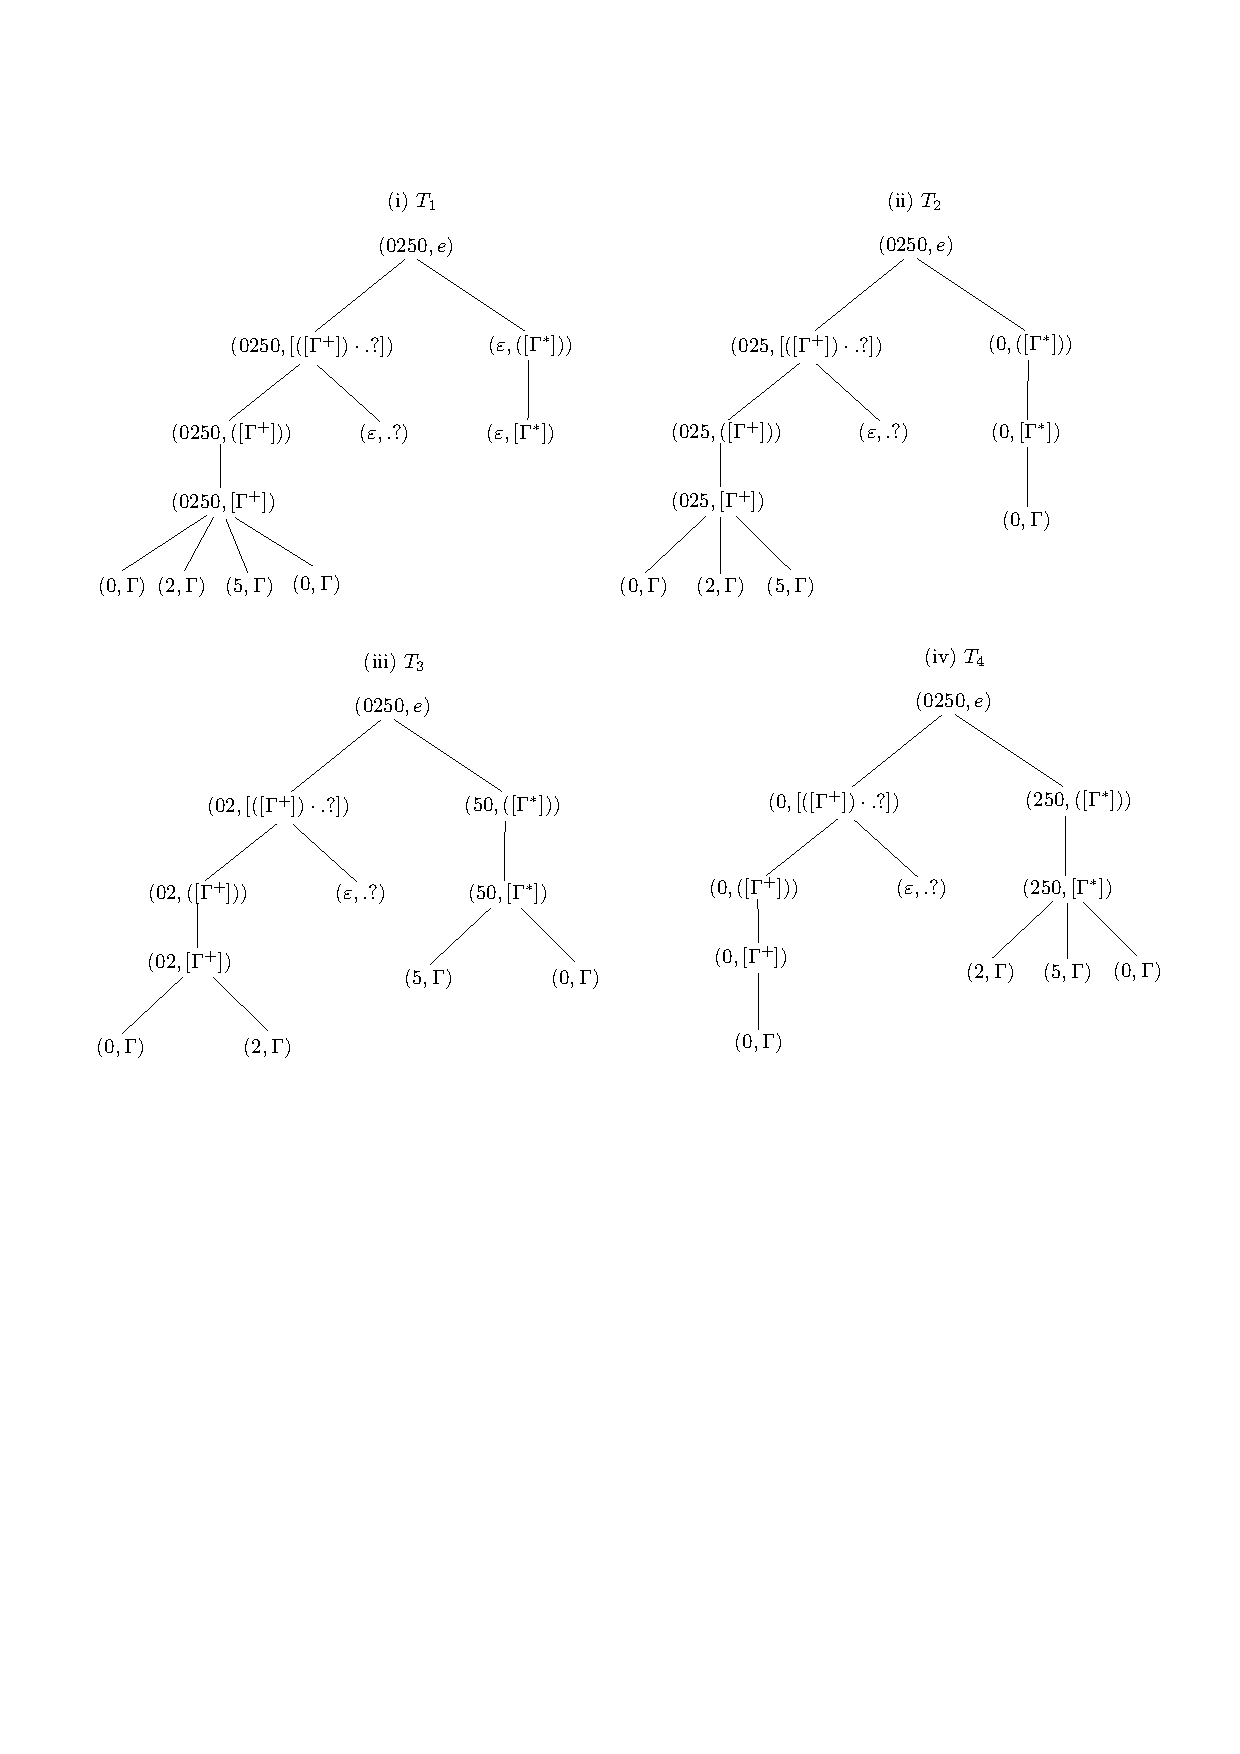
\includegraphics[width=1\textwidth]{regex-semantics-decimal.pdf}
\caption{Match trees of $e=[[([\Gamma^+])\concat .?] \concat ([\Gamma^*])]$ to $w= 0250$}
\label{fig-regex-semantics-decimal}

\end{figure}
%\Blindtext
 \end{example}



%%%%% the original example %%%%%%%%%%
%%%%% the original example %%%%%%%%%%
\hide{  
\begin{example}\label{exmp-regex-match-tree}
Let $e = ((b^\ast) \cdot ((b \cdot a^\ast) | \varepsilon)) \cdot a^\ast$ and $w= baa$. Then $\cM_{w}(e) = \{T_1,T_2,T_3\}$ as illustrated in Figure~\ref{fig-regex-semantics}: (i), (ii), (iii).  
\begin{figure}[ht]
\centering
%\rule{\linewidth}{0cm}
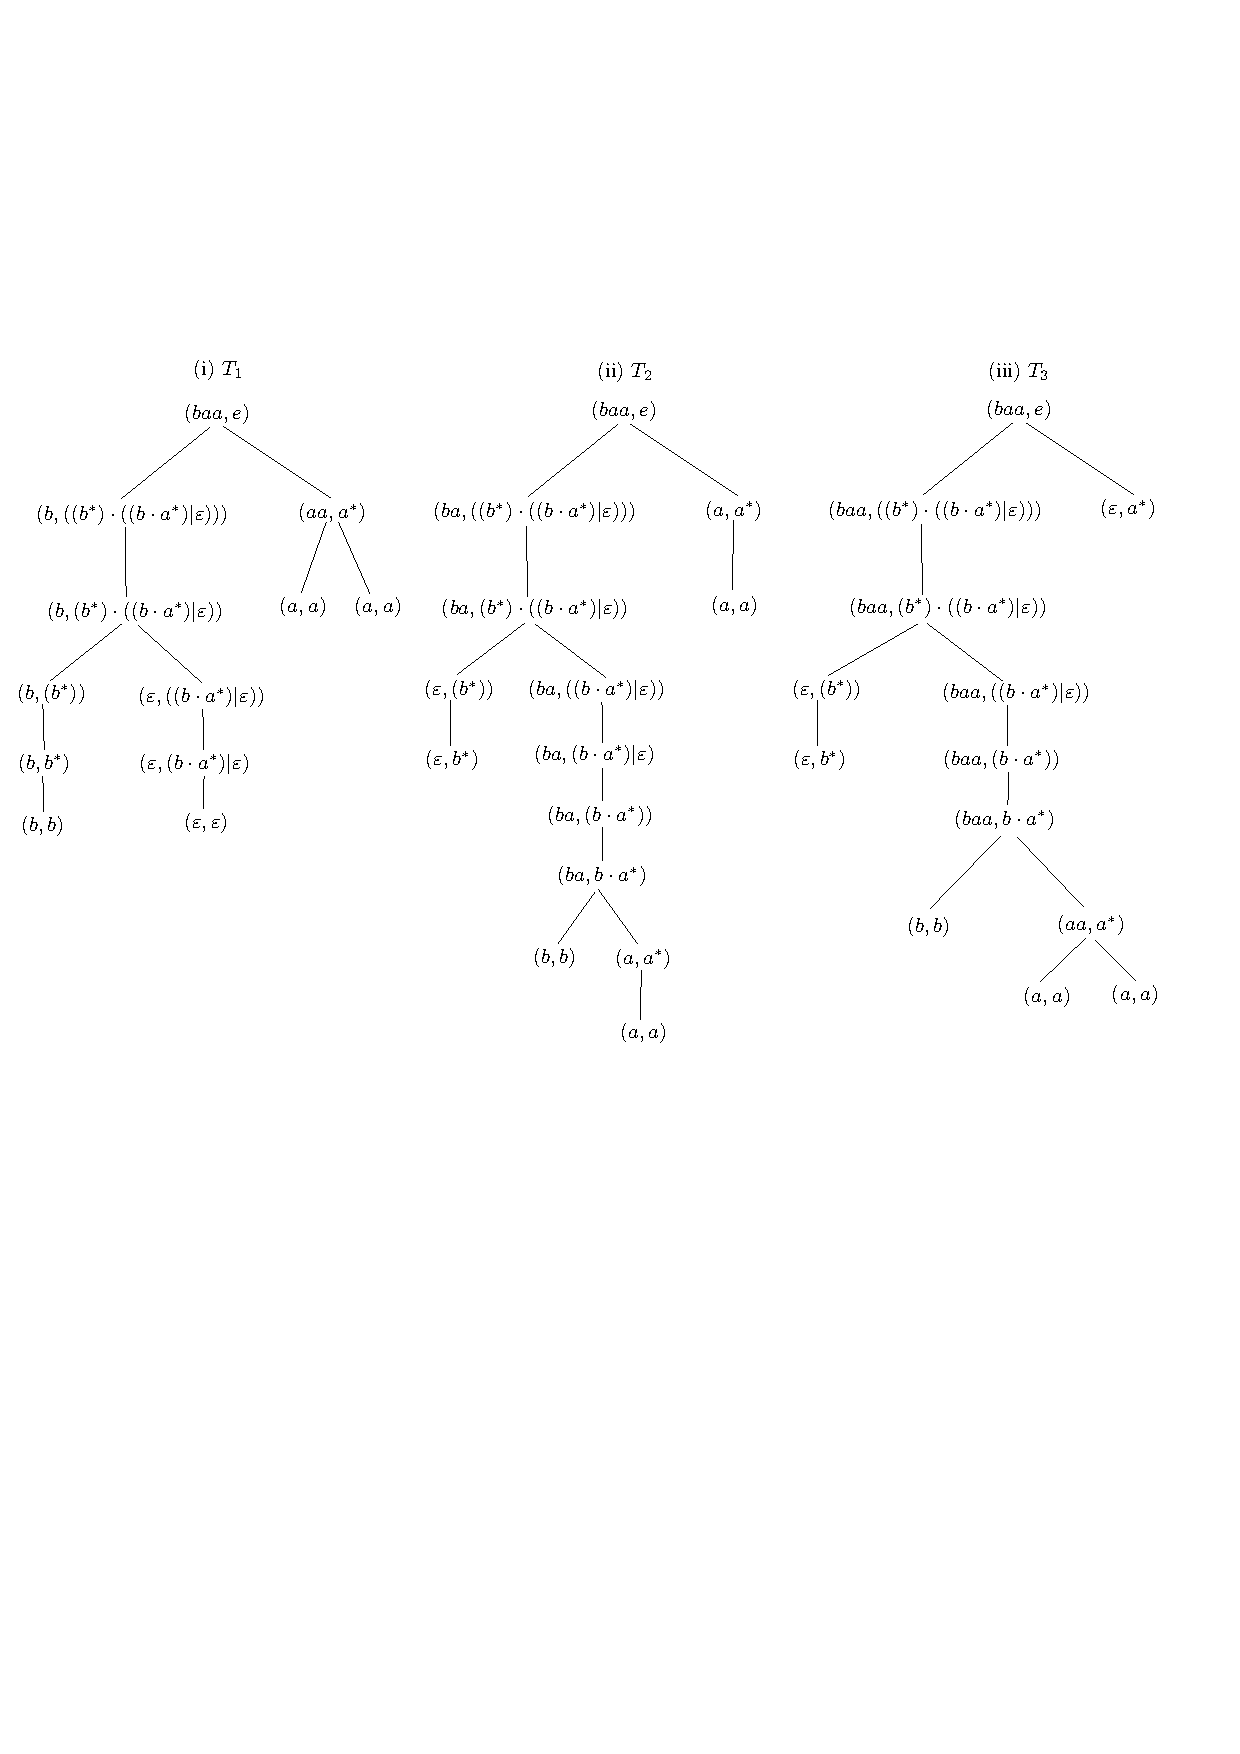
\includegraphics[width=1\textwidth]{regex-semantics.pdf}
\caption{Match trees of $e=((b^\ast) \cdot ((b \cdot a^\ast) | \varepsilon)) \cdot a^\ast$ to $w= baa$}
\label{fig-regex-semantics}
\end{figure}
%\Blindtext
 \end{example}
 }
 %%%%% the original example %%%%%%%%%%
%%%%% the original example %%%%%%%%%% 
  
  \begin{definition}[Semantics of $\regexp$]\label{def-regex-semantics}
  	For a $\regexp$ $e$ and a string $w$, we recursively define a (strict) total order on $\cM_{\pref(w)}(e)$, written $T
  	>_{w,\idxexp(e)} T'$ for $T, T' \in \cM_{\pref(w)}(e)$, as follows:
  	\begin{itemize}
  		\item $\idxexp(e) = \varepsilon$, $\idxexp(e) = a$, or $\idxexp(e) = \$ n$. There is only one match tree, thus the
  		order $>_{w, \idxexp(e)}$ is empty. %\tl{this is nitpicking, but linear order implies reflectivity }\zhilin{changed to strict total order}
 %
 		\item $\idxexp(e)  = [e_1?]$. 
 		
 		\begin{itemize}
            \item If $T' $ is  a single node $(\varepsilon, \idxexp(e))$, but $T$ is not, then $T >_{w, \idxexp(e)} T'$.
            
  			\item If $C (T) = (w_1, e_1)$ and $C (T') = (w_2, e_1)$ for some $w_1, w_2 \in \pref(w)$, then $T >_{w, \idxexp(e)} T'$ iff $T_{(w_1, e_1)} >_{w, e_1} T'_{(w_2, e_1)}$.
 		\end{itemize}
 		
 		\item $\idxexp(e)  = [e_1??]$. 
 		
 		\begin{itemize}
            \item If $T $ is  a single node $(\varepsilon, \idxexp(e))$, but $T'$ is not, then $T >_{w, \idxexp(e)} T'$.
%  			
  			\item If $C (T) = (w_1, e_1)$ and $C (T') = (w_2, e_1)$ for some $w_1, w_2 \in \pref(w)$, then $T >_{w, \idxexp(e)} T'$ iff $T_{(w_1, e_1)} >_{w, e_1} T'_{(w_2, e_1)}$.
 		\end{itemize}

  		\item $\idxexp(e) = (_n e_1)_n$. Suppose that $C (T) = (w_1, e_1)$ and $C (T') = (w_2, e_1)$ for some $w_1, w_2 \in \pref(w)$.
  		Then $T >_{w, \idxexp(e)} T'$ iff $T_{(w_1, e_1)} >_{w, e_1} T'_{(w_2, e_1)}$.
  		
  		\item $\idxexp(e) = [e_1 + e_2]$.
  		\begin{itemize}
  			\item If $C (T) = (w_1, e_1)$ and $C (T') = (w_2, e_2)$ for some $w_1, w_2 \in \pref(w)$, then $T >_{w, \idxexp(e)} T'$.
%  			
  			\item If $C (T) = (w_i, e_i)$ and $C (T') = (w'_i, e_i)$ for some $i \in \{ 1,
  			2 \}$ and $w_i, w'_i \in \pref(w)$, then $T >_{w, \idxexp(e)} T'$ iff $T_{(w_i, e_i)} >_{w, e_i} T'_{(w'_i, e_i)}$.
  		\end{itemize}
  		\item $\idxexp(e) = [e_1 \cdot e_2]$. Suppose $C (T) = (w_1, e_1) (w_2, e_2)$ and $C (T') =
  		(w_1', e_1) (w_2', e_2)$ (note that $w_1$ is a prefix of $w'_1$ or vice versa), then $T >_{w, \idxexp(e)} T'$ when either $T_{(w_1, e_1)} >_{w, e_1}
  		T'_{(w_1', e_1)}$, or $w_1 = w_1'$ and $T_{(w_2, e_2)} >_{w_1^{-1}w, e_2} T'_{(w_2', e_2)}$. 
%  		
  		\item $\idxexp(e) = [e_1^{\ast}]$. 
		\begin{itemize}
		\item If $T' $ is  a single node $(\varepsilon, \idxexp(e))$, but $T$ is not, then $T >_{w, \idxexp(e)} T'$.
  		\item Otherwise, suppose $C(T) = (w_1, e_1) \ldots (w_k, e_1)$ and $C (T') = (w_1', e_1)$ $\ldots$ $(w_l', e_1)$, we have $T >_{w, \idxexp(e)} T'$ iff either $k > l$ and for every $i \in [l]$ we have $T_{(w_j, e_1)} = T_{(w_j', e_1)}$, or for the first index $j$ such that $T_{(w_j, e_1)} \neq T_{(w_j', e_1)}$, we have $T_{(w_j, e_1)}$ $>_{(w_1\cdots w_{j-1})^{-1}w, e_1}$ $T'_{(w_j', e_1)}$.
		\end{itemize}
%
  		\item $\idxexp(e) = [e_1^{+}]$ or $[e_1^{\{m_1, m_2\}}]$. 
  		Suppose $C(T) = (w_1, e_1) \ldots (w_k, e_1)$ and $C (T') = (w_1', e_1)$ $\ldots$ $(w_l', e_1)$, then $T >_{w, \idxexp(e)} T'$ iff either $k > l$ and for every $i \in [l]$ we have $T_{(w_j, e_1)} = T_{(w_j', e_1)}$, or for the first index $j$ such that $T_{(w_j, e_1)} \neq T_{(w_j', e_1)}$, we have $T_{(w_j, e_1)}$ $>_{(w_1\cdots w_{j-1})^{-1}w, e_1}$ $T'_{(w_j', e_1)}$.
%
  		\item $\idxexp(e) = [e_1^{\ast?}]$. 
		\begin{itemize}
		\item If $T$ is a single node  $(\varepsilon, \idxexp(e))$, but $T'$ is not, then $T >_{w, \idxexp(e)} T'$.
  		\item Otherwise, suppose $C(T) = (w_1, e_1) \ldots (w_k, e_1)$ and $C (T') =
  		(w_1', e_1)$ $\ldots$ $(w_l', e_1)$, we have $T >_{w, \idxexp(e)} T'$ iff either $k < l$ and for every $i \in [k]$ we have $T_{(w_j, e_1)} = T_{(w_j', e_1)}$, or for the first index $j$ such that $T_{(w_j, e_1)} \neq T_{(w_j', e_1)}$, we have $T_{(w_j, e_1)}$ $>_{(w_1\cdots w_{j-1})^{-1}w, e_1}$ $T'_{(w_j', e_1)}$.
		\end{itemize}
%
  		\item $\idxexp(e) = [e_1^{+?}]$ or $[e_1^{\{m_1, m_2\}?}]$. 
  		Suppose $C(T) = (w_1, e_1) \ldots (w_k, e_1)$ and $C (T') = (w_1', e_1)$ $\ldots$ $(w_l', e_1)$, then $T >_{w, \idxexp(e)} T'$ iff either $k < l$ and for every $i \in [k]$ we have $T_{(w_j, e_1)} = T_{(w_j', e_1)}$, or for the first index $j$ such that $T_{(w_j, e_1)} \neq T_{(w_j', e_1)}$, we have $T_{(w_j, e_1)}$ $>_{(w_1\cdots w_{j-1})^{-1}w, e_1}$ $T'_{(w_j', e_1)}$.

  	\end{itemize}
  	
  	For $e \in \regexp$ and $w \in \Lang(e)$, the \emph{accepting match} of $e$ to $w$, denoted by $M_e(w)$, is the supremum of $\cM_w(e)$.
  	 Moreover,  for $e \in \regexp$ and $w \in \Sigma^\ast$, if $w \in \Sigma^\ast \Lang(e)\Sigma^\ast$, then the (first) \emph{match} of $e$ in $w$ is defined as the supremum of $\cM_{\pref(w_1^{-1}w)}(e)$ such that $w_1$ is the shortest prefix of $w$ satisfying that $w_1^{-1}w \in \Lang(e)\Sigma^\ast$. If $w \not \in \Sigma^\ast \Lang(e)\Sigma^\ast$, the match of $e$ in $w$ is undefined.  
  	%\tl{why do we need this extra def?}\zhilin{to define the semantics of replace function for instance.}
%  	
%  	For any subexpression $e'$ of $e$, suppose $(w_1, e') \ldots (w_m, e')$ are
%  	all the nodes labeled by $(w', e')$ with $w' \neq \varepsilon$, in the
%  	pre-order traversal of $M_e(w)$. Then the match result captured by $e'$, denoted
%  	by $M_{e', e} (w)$, is the sequence of substrings $w_1 \ldots w_m$.
  \end{definition}

\begin{example}\label{exmp-regex-semantics}
Let us continue Example~\ref{exmp-regex-match-tree}.  In Fig.~\ref{fig-regex-semantics-decimal}, we have $(T_1)_{(0250, [\Gamma^+])} >_{(w, \idxexp(e))} (T_2)_{(025, [\Gamma^+])}$, since $(0, \Gamma)(2, \Gamma)(5,\Gamma)$ is a proper prefix of $(0, \Gamma)(2, \Gamma)(5,\Gamma)(0, \Gamma)$. Then we deduce that $(T_1)_{(0250, (_1[\Gamma^+])_1)} >_{(w, \idxexp(e))} (T_2)_{(025, (_1[\Gamma^+])_1)}$. Consequently, $(T_1)_{(0250, [(_1[\Gamma^+])_1 \concat .?])} >_{(w, \idxexp(e))} (T_2)_{(025,  [(_1[\Gamma^+])_1 \concat .?])}$ and $T_1 >_{(w, \idxexp(e))} T_2$. Similarly, we have $T_2 >_{(w, \idxexp(e))} T_3$ and $T_3 >_{(w, \idxexp(e))} T_4$. Therefore, $T_1$ is the accepting match of $e$ to $w$, where the first and second capturing group of $e$ are matched to $0250$  and $\varepsilon$ respectively. 
%\Blindtext
 \end{example}
  
\begin{remark}
Our semantics of $\regexp$ follows the 11th Edition of the ECMAScript specification (ES11 for short) \cite{ECMAScript11}, with a focus on the non-commutative union, the greedy/lazy semantics of Kleene star/plus, as well as capturing groups and backreferences.
In comparison, POSIX regular expressions require the leftmost and longest match of regular expressions, which we leave as future work.
\end{remark}
  
  
% some examples
  
%  e = b(a*)a*
%  
%  e' = b(a*?)a*
